\documentclass{standalone}
\usepackage{tikz}
\begin{document}
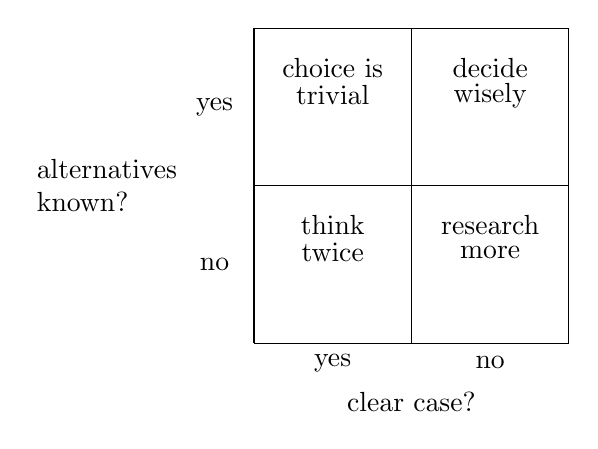
\begin{tikzpicture}[scale=0.5]
        \node at (-4,4) {\parbox{10ex}{alternatives known?}};
        % \node at (-4,3.3) {\emph{do we know it?}};
            \node at (-1,2) {no};
            \node at (-1,6) {yes};
        \node at (4,-1.5) {clear case?};
        % \node at (4,-2.2) {\emph{do we know whether we know it?}};
            \node at (2,-0.5) {yes};
            \node at (6,-0.5) {no};
        \draw (0,0) -- (0,8) -- (8,8) -- (8,0) -- (0,0);
        \draw (4,0) -- (4,8) ; \draw (0,4) -- (8,4);
        
        \node at (2,3) {think};
            \node at (2,2.3) {twice};
            
        \node at (2,7) {choice is};
            \node at (2,6.3) {trivial};
            
        \node at (6,3) {research};
            \node at (6,2.3) {more};
            
        \node at (6,7) {decide};
            \node at (6,6.3) {wisely};
\end{tikzpicture}
\end{document}